\section*{Materials and methods}

\subsection*{Data}

We tested AFQ-Insight in a classification setting using data from a previous study of the corticospinal tract profile in patients with amyotrophic lateral sclerosis (ALS)\cite{sarica2017corticospinal}. This study collected dMRI data from 24 ALS patients and 24 demographically matched healthy controls. In the regression setting, we used dMRI data from a previous study of properties of the white matter across the lifespan\cite{yeatman2014lifespan}, containing dMRI data from 76 subjects with ages 6-50. In both cases, the authors of these previous studies made their imaging data available through\ldots \adam{How? Through neurovault? Private correspondence?}.

The ``raw'' dMRI data from the ALS and lifespan maturation studies were then analyzed using the Automated Fiber-Tract Quantification tractometry pipeline\cite{yeatman2012tract} with the pyAFQ package\cite{pyAFQ} \adam{Or was it the MATLAB implementation?}. This creates tract profiles, in which diffusion measures are quantified and averaged along twenty major fiber tracts. These tract profiles, along with the phenotypical data we wish to explain or predict, form the input to AFQ-Insight. In a domain-agnostic machine learning context, the phenotypical data comprise the target variables while the tract profiles form the feature or predictor variables.

AFQ-Insight reads the target and feature data from comma separated value (CSV) files conforming to the AFQ-Browser data format\cite{yeatman2018browser} \adam{Should we cite the specific page in the online documentation} and represents them internally as \lstinline{DataFrame} objects from the pandas Python library\cite{mckinney2010data}. We leave imputation of the target data to the user and automatically impute missing data only in the feature matrix. Missing interior nodes are imputed using linear interpolation. For missing exteriod nodes, the user may choose between linear extrapolation and constant forward(back)-fill. The data imputation uses only values from adjacent nodes in the same white matter tract in the same subject so there is no danger of data leakage from other subjects.

Lastly, like most learning algorithms, AFQ-Insight benefits from standardization of the input dataset. Some diffusion metrics will have naturally larger variance than others and may therefore dominate the objective function and make the sparse group lasso estimator unable to learn from the lower variance metrics. For example, fractional anisotropy (FA) is bounded between zero and one and could be overwhelmed by an unscaled higher-variance metric like the mean diffusivity (MD). To prevent this, AFQ-Insight uses the \lstinline{StandardScaler} from scikit-learn\cite{scikit-learn}, to remove each feature's mean and scale it to unit variance. Scaling is performed separately within each cross-validation set's training or testing data to prevent leakage of information between the testing and training sets\cite{kaufman2012leakage}.

\subsection*{Sparse Group Lasso}

After scaling and imputation, the tractometry data and target phenotypical data can be organized in a linear model, $y = \mathbf{X} \cdot \beta$, where $y$ is the phenotype -- categorical, such as a clinical diagnosis, or numerical, such as the subject's age. The tractometry data is represented in the feature matrix $\mathbf{X}$, with rows corresponding to different subjects, and columns corresponding to diffusion measures at different nodes within each tract. The relationship between tractometric features and the phenotypic target is characterized by the coefficients in $\beta$. The feature matrix $\mathbf{X}$ has dimensions $N_s \times (N_t \cdot N_n \cdot N_m)$, where $N_s$ is the number of subjects, $N_t$ is the number of white matter tracts, $N_n$ is the number of nodes in each tract, and $N_m$ is the number of diffusion metrics calculated at each node. Typically, $N_t = 20$, $N_n = 100$, and $2 \le N_m \le 8$, resulting in $\mathcal{O}(10^4)$ features. Conversely, most dMRI studies have $\mathcal{O}(10^2)$ participants, yielding a feature matrix that is wide and short. The high dimensionality of this data requires regularization to avoid overfitting and generate interpretable results.

In addition to regularizing the coefficients in $\beta$, we also wish to capitalize upon our knowledge of the group structure of the tract profile features in $\mathbf{X}$. The tract-metric combinations form a natural grouping. For example, we expect that MD features within the left arcuate fasciculus will be correlated. Likewise for FA values within the right corticospinal tract (CST) and so on. This group structure is represented in Fig~\ref{fig:group-structure}, which depicts the linear model $y = \mathbf{X} \cdot \beta$. The target vector $y$ is sorted into patients (p) and controls (c), while the different colors encode the group structure of the feature matrix $\mathbf{X}$, with one group for each unique tract-metric combination.

\begin{figure}[!h]
    \centering
    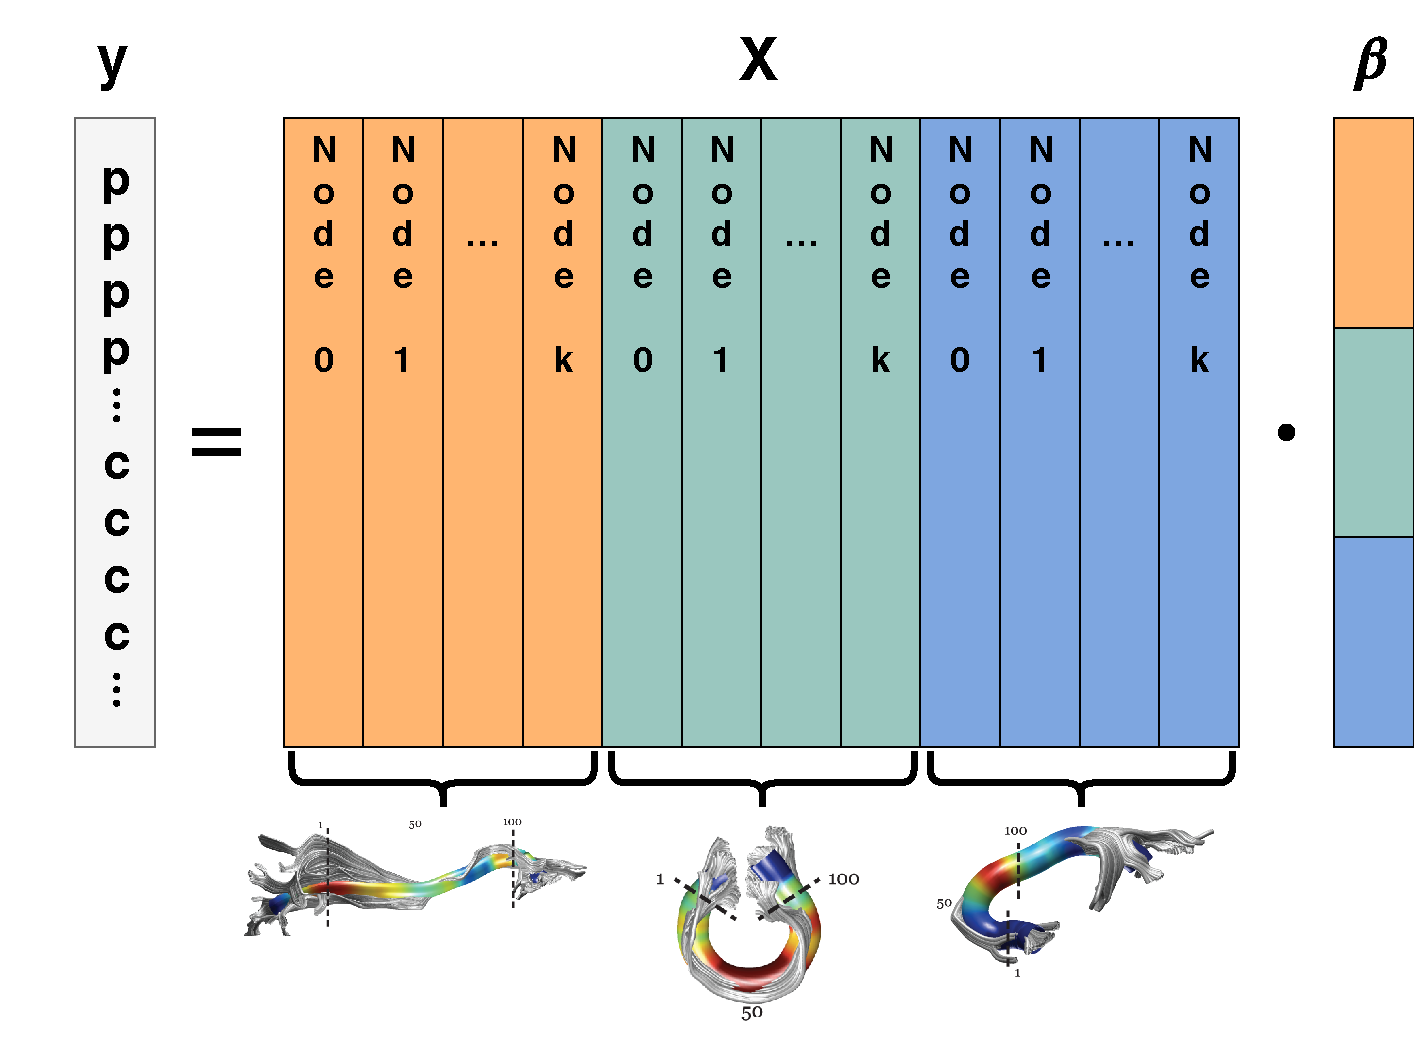
\includegraphics[width=0.65\textwidth]{dMRI_group_structure.pdf}
    \caption{{\bf dMRI group structure.}
        The phenotypical target data and tractometric features can be organized into a linear model, $y = \mathbf{X} \cdot \beta$. Here, the target array $y$ is suggestively sorted into patients (p) and controls (c), while the feature matrix $\mathbf{X}$ is color-coded to reveal a natural group structure. In this example, the left (orange) group contains $k$ features from the inferior fronto-occipital fascicle (IFOF), the middle (green) group contains $k$ features from the corpus callosum, and the right (blue) group contains $k$ features from the uncinate. The coefficients in $\beta$ follow the same natural grouping. Fascicle images taken with permission from Ref~\cite{yeatman2012tract}.
    }
    \label{fig:group-structure}
\end{figure}

Thus, we seek a regularization approach that will fit a linear model with anatomically-grouped covariates, where we expect to observe sparse coefficients at both the group level and the within-group level. The sparse group lasso (SGL) is a penalized regression technique that satisfies exactly these criteria\cite{simon2013sparse}. It solves for a coefficient vector $\widehat{\beta}$ that satisfies
\begin{equation}
    \widehat{\beta} = \min_\beta \frac{1}{2}
    \norm*{y - \displaystyle \sum_{\ell = 1}^{m} \mathbf{X}^{(\ell)} \cdot \beta^{(\ell)}}_2^2
    + \lambda_1 \displaystyle \sum_{\ell = 1}^{m} \sqrt{p_\ell} \norm*{\beta^{(\ell)}}_2
    + \lambda_2 \norm*{\beta}_1,
    \label{eq:sgl}
\end{equation}
where $m$ is the number of anatomical groups, $\mathbf{X}^{(\ell)}$ is the submatrix of $\mathbf{X}$ corresponding to group $\ell$, $\beta^{(\ell)}$ is the coefficient vector for group $\ell$ and $p_\ell$ is the length of $\beta^{(\ell)}$. The first term is the mean square error loss, $L_{mse}$, as in the standard linear regression framework. The second and third terms encourage groupwise sparsity and overall sparsity, respectively. If $\lambda_1 = 0$ and $\lambda_2 = 1$, the SGL reduces to the traditional lasso\cite{tibshirani1996regression}. Conversely, if $\lambda_1 = 1$ and $\lambda_2 = 0$, the SGL reduces to the group lasso\cite{yuan2006model}.

When the phenotypical target variable are categorical, as in the case of predicting a clinical diagnosis, the SGL is readily adapted to logistic regression, where the probability of a target variable belonging to an arbitrary defined ``true'' class is the logistic function of the result of the linear model,
\begin{equation}
    p(y = 1) = \frac{1}{1 + \exp(\mathbf{X}\cdot \beta)},
    \label{eq:logit}
\end{equation}
or equivalently, the mean squared error loss function in Eq~\eqref{eq:sgl} is replaced with the cross-entropy loss, which for binary classification is the negative log likelihood of the SGL classifier giving the ``true'' label:
\begin{equation}
    L_{mse} \rightarrow L_{\log} = -\left(y \log(p) + (1 - y) \log(1 - p)\right).
    \label{eq:logloss}
\end{equation}

\begin{itemize}
  \item Computational implementation
    \begin{itemize}
      \item Insert Figure for pipeline
      \item Proximal gradient methods
      \item Meta-parameter optimization
      \item Cross-validation scheme
        \begin{itemize}
          \item Insert Figure for cross-validation scheme
        \end{itemize}
    \end{itemize}
\end{itemize}
